\documentclass[journal,12pt,twocolumn]{IEEEtran}
%
\usepackage{setspace}
\usepackage{gensymb}
\usepackage{xcolor}
%\usepackage{esint}
\usepackage{caption}
%\usepackage{subcaption}
%\doublespacing
\singlespacing
\usepackage{multicol}

\usepackage{iithtlc}
%\usepackage{graphicx}
%\usepackage{amssymb}
%\usepackage{relsize}
\usepackage[cmex10]{amsmath}
\usepackage{mathtools}
%\usepackage{amsthm}
%\interdisplaylinepenalty=2500
%\savesymbol{iint}
%\usepackage{txfonts}
%\restoresymbol{TXF}{iint}
%\usepackage{wasysym}
\usepackage{amsthm}
\usepackage{mathrsfs}
\usepackage{txfonts}
\usepackage{stfloats}
\usepackage{cite}
\usepackage{cases}
\usepackage{subfig}
%\usepackage{xtab}
\usepackage{longtable}
\usepackage{multirow}
%\usepackage{algorithm}
%\usepackage{algpseudocode}
\usepackage{enumerate}
\usepackage{mathtools}
%\usepackage{stmaryrd}

\usepackage{listings}
%    \usepackage[latin]{inputenc}                                 %%
    \usepackage{color}                                            %%
    \usepackage{array}                                            %%
    \usepackage{longtable}                                        %%
    \usepackage{calc}                                             %%
    \usepackage{multirow}                                         %%
    \usepackage{hhline}                                           %%
    \usepackage{ifthen}                                           %%
  %optionally (for landscape tables embedded in another document): %%
    \usepackage{lscape}   
    \usepackage{tikz}
\usetikzlibrary{calc}
\usepackage{tkz-euclide}
\usetkzobj{all}
  
%\usepackage{tikz}
%\usepackage{tkz-euclide}
%\usetkzobj{all}
%%\usepackage[utf8]{inputenc}
%\usepackage{rotating}
%\usetikzlibrary{arrows,shapes,decorations.markings,positioning}
%\usepackage{amsmath}
%\usepackage{ulem}
%\usepackage{soul}

%\usepackage{wasysym}
%\newcounter{MYtempeqncnt}
\DeclareMathOperator*{\Res}{Res}
%\renewcommand{\baselinestretch}{2}
\renewcommand\thesection{\arabic{section}}
\renewcommand\thesubsection{\thesection.\arabic{subsection}}
\renewcommand\thesubsubsection{\thesubsection.\arabic{subsubsection}}

\renewcommand\thesectiondis{\arabic{section}}
\renewcommand\thesubsectiondis{\thesectiondis.\arabic{subsection}}
\renewcommand\thesubsubsectiondis{\thesubsectiondis.\arabic{subsubsection}}

%\DeclareUnicodeCharacter{01B5}{\zst}
%\DeclareRobustCommand\zst{%
%\unskip\nobreak\thinspace\zbar\allowbreak\thinspace\ignorespaces}
%\newcommand{\zbar}{\raisebox{0.2ex}{--}\kern-0.6em Z}


% correct bad hyphenation here
\hyphenation{op-tical net-works semi-conduc-tor}

\def\inputGnumericTable{}  

\lstset{
language=python,
frame=single, 
breaklines=true
}

\begin{document}
%

\theoremstyle{definition}
\newtheorem{theorem}{Theorem}[section]
\newtheorem{problem}{Problem}
\newtheorem{proposition}{Proposition}[section]
\newtheorem{lemma}{Lemma}[section]
\newtheorem{corollary}[theorem]{Corollary}
\newtheorem{example}{Example}[section]
\newtheorem{definition}{Definition}[section]
%\newtheorem{algorithm}{Algorithm}[section]
%\newtheorem{cor}{Corollary}
\newcommand{\BEQA}{\begin{eqnarray}}
\newcommand{\EEQA}{\end{eqnarray}}
\newcommand{\define}{\stackrel{\triangle}{=}}

\bibliographystyle{IEEEtran}
%\bibliographystyle{ieeetr}



\providecommand{\pr}[1]{\ensuremath{\Pr\left(#1\right)}}
\providecommand{\qfunc}[1]{\ensuremath{Q\left(#1\right)}}
\providecommand{\sbrak}[1]{\ensuremath{{}\left[#1\right]}}
\providecommand{\lsbrak}[1]{\ensuremath{{}\left[#1\right.}}
\providecommand{\rsbrak}[1]{\ensuremath{{}\left.#1\right]}}
\providecommand{\brak}[1]{\ensuremath{\left(#1\right)}}
\providecommand{\lbrak}[1]{\ensuremath{\left(#1\right.}}
\providecommand{\rbrak}[1]{\ensuremath{\left.#1\right)}}
\providecommand{\cbrak}[1]{\ensuremath{\left\{#1\right\}}}
\providecommand{\lcbrak}[1]{\ensuremath{\left\{#1\right.}}
\providecommand{\rcbrak}[1]{\ensuremath{\left.#1\right\}}}
\theoremstyle{remark}
\newtheorem{rem}{Remark}
\newcommand{\sgn}{\mathop{\mathrm{sgn}}}
\providecommand{\abs}[1]{\left\vert#1\right\vert}
\providecommand{\res}[1]{\Res\limits_{#1}} 
\providecommand{\norm}[1]{\lVert#1\rVert}
\providecommand{\mtx}[1]{\mathbf{#1}}
\providecommand{\mean}[1]{E\left[ #1 \right]}
\providecommand{\fourier}{\overset{\mathcal{F}}{ \rightleftharpoons}}
%\providecommand{\hilbert}{\overset{\mathcal{H}}{ \rightleftharpoons}}
\providecommand{\system}{\overset{\mathcal{H}}{ \longleftrightarrow}}
\providecommand{\gauss}[2]{\mathcal{N}\ensuremath{\left(#1,#2\right)}}
	%\newcommand{\solution}[2]{\textbf{Solution:}{#1}}
\newcommand{\solution}{\noindent \textbf{Solution: }}
\providecommand{\dec}[2]{\ensuremath{\overset{#1}{\underset{#2}{\gtrless}}}}
%\numberwithin{equation}{section}
%\numberwithin{problem}{section}
\makeatletter
\@addtoreset{figure}{problem}
\makeatother

\let\StandardTheFigure\thefigure
%\renewcommand{\thefigure}{\theproblem.\arabic{figure}}
\renewcommand{\thefigure}{\theproblem}

\def\putbox#1#2#3{\makebox[0in][l]{\makebox[#1][l]{}\raisebox{\baselineskip}[0in][0in]{\raisebox{#2}[0in][0in]{#3}}}}
     \def\rightbox#1{\makebox[0in][r]{#1}}
     \def\centbox#1{\makebox[0in]{#1}}
     \def\topbox#1{\raisebox{-\baselineskip}[0in][0in]{#1}}
     \def\midbox#1{\raisebox{-0.5\baselineskip}[0in][0in]{#1}}


% paper title
% can use linebreaks \\ within to get better formatting as desired
\title{
\logo{
GATE problems in Complex Analysis
}
}
%
%
% author names and IEEE memberships
% note positions of commas and nonbreaking spaces ( ~ ) LaTeX will not break
% a structure at a ~ so this keeps an author's name from being broken across
% two lines.
% use \thanks{} to gain access to the first footnote area
% a separate \thanks must be used for each paragraph as LaTeX2e's \thanks
% was not built to handle multiple paragraphs
%

%\author{Y Aditya, A Rathnakar and G V V Sharma$^{*}$% <-this % stops a space
%\author{G V V Sharma$^{*}$% <-this % stops a space
%\thanks{*The author is with the Department
%of Electrical Engineering, Indian Institute of Technology, Hyderabad
%502205 India e-mail:  gadepall@iith.ac.in.All content in this manual is released under GNU GPL.  Free and open source.}% <-this % stops a space
%%\thanks{J. Doe and J. Doe are with Anonymous University.}% <-this % stops a space
%%\thanks{Manuscript received April 19, 2005; revised January 11, 2007.}}
%}
% note the % following the last \IEEEmembership and also \thanks - 
% these prevent an unwanted space from occurring between the last author name
% and the end of the author line. i.e., if you had this:
% 
% \author{....lastname \thanks{...} \thanks{...} }
%                     ^------------^------------^----Do not want these spaces!
%
% a space would be appended to the last name and could cause every name on that
% line to be shifted left slightly. This is one of those "LaTeX things". For
% instance, "\textbf{A} \textbf{B}" will typeset as "A B" not "AB". To get
% "AB" then you have to do: "\textbf{A}\textbf{B}"
% \thanks is no different in this regard, so shield the last } of each \thanks
% that ends a line with a % and do not let a space in before the next \thanks.
% Spaces after \IEEEmembership other than the last one are OK (and needed) as
% you are supposed to have spaces between the names. For what it is worth,
% this is a minor point as most people would not even notice if the said evil
% space somehow managed to creep in.



% The paper headers
%\markboth{Journal of \LaTeX\ Class Files,~Vol.~6, No.~1, January~2007}%
%{Shell \MakeLowercase{\textit{et al.}}: Bare Demo of IEEEtran.cls for Journals}
% The only time the second header will appear is for the odd numbered pages
% after the title page when using the twoside option.
% 
% *** Note that you probably will NOT want to include the author's ***
% *** name in the headers of peer review papers.                   ***
% You can use \ifCLASSOPTIONpeerreview for conditional compilation here if
% you desire.




% If you want to put a publisher's ID mark on the page you can do it like
% this:
%\IEEEpubid{0000--0000/00\$00.00~\copyright~2007 IEEE}
% Remember, if you use this you must call \IEEEpubidadjcol in the second
% column for its text to clear the IEEEpubid mark.



% make the title area
\maketitle

%\tableofcontents

\begin{abstract}
This manual has problems on Complex Analysis taken from GATE papers in Mathematics and Electronics and Communication Engineering. 
%
\end{abstract}
% IEEEtran.cls defaults to using nonbold math in the Abstract.
% This preserves the distinction between vectors and scalars. However,
% if the journal you are submitting to favors bold math in the abstract,
% then you can use LaTeX's standard command \boldmath at the very start
% of the abstract to achieve this. Many IEEE journals frown on math
% in the abstract anyway.

% Note that keywords are not normally used for peerreview papers.
%\begin{IEEEkeywords}
%Cooperative diversity, decode and forward, piecewise linear
%\end{IEEEkeywords}



% For peer review papers, you can put extra information on the cover
% page as needed:
% \ifCLASSOPTIONpeerreview
% \begin{center} \bfseries EDICS Category: 3-BBND \end{center}
% \fi
%
% For peerreview papers, this IEEEtran command inserts a page break and
% creates the second title. It will be ignored for other modes.
\IEEEpeerreviewmaketitle


%\newpage
%\section{Two Variable}
%
%\subsection{Multivariate Gaussian}
%
%\renewcommand{\thefigure}{Q\theenumi(\theenumii)}
\renewcommand{\thefigure}{\theenumi}
\begin{enumerate}[1.]
\item The contour $C$ given below is on the complex plane $z = x + \j y$.
Find the value of the integral $\dfrac{1}{\pi\j}\oint\limits_{C}\dfrac{dz}{z^2-1}$.
%
\begin{figure}[!h]
\centering
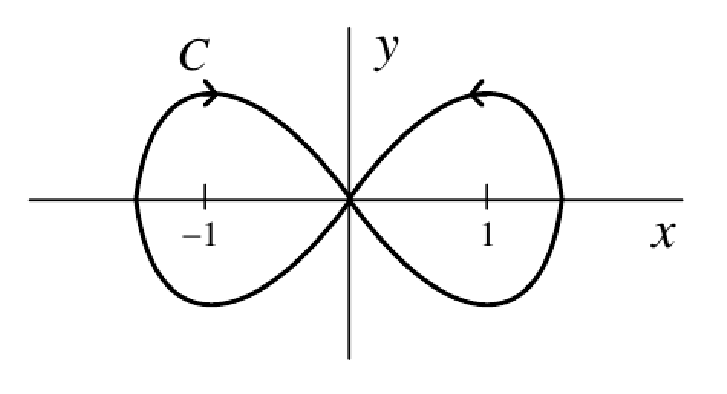
\includegraphics[width=\columnwidth]{./figs/ec2018.eps}
\caption{}
\label{fig:ec2018}
\end{figure}
\item An integral $I$  is given by 
\begin{equation}
I = \ointctrclockwise\limits_{C}\frac{z^2-1}{z^2+1} e^z\,dz.
\end{equation}
If $C: \abs{z} = 3$, find the value of $I$.
%\item Let $C:\abs{z} = 1$.  Find
%\begin{equation}
%\ointctrclockwise_{C}xy^2\,dx+x^2y\,dy
%\end{equation}
\item Consider contour integration performed over $C:\abs{z} = 1$ in the anticlockwise direction.  Which of the following is
NOT true?
\begin{enumerate}
\setlength\itemsep{0.5em}
\item The residue of $\frac{z}{z^2-1}$ at $z = 1$ is $\frac{1}{2}$.
\item $\ointctrclockwise\limits_{C}z^2\,dz = 0$
\item $\frac{1}{2\pi\j}\ointctrclockwise\limits_{C}\frac{dz}{z}= 1$.
\item $\bar{z}$ is an analytic function.
\end{enumerate}
\item Find the value of 
\begin{equation}
\ointctrclockwise\limits_{C}\frac{z^2-z+4\j}{z+2\j}\,dz, \quad C:\abs{z} = 3.
\end{equation}
\item Given 
\begin{equation}
f(z) = \frac{1}{z+1}-\frac{2}{z+3}.
\end{equation}
%
If $\abs{z+1} = 1 $, find $\frac{1}{2\pi\j}\ointctrclockwise\limits_{C}f(z)\,dz$.
\item Find 
\begin{equation}
\ointctrclockwise\limits_{C}\frac{-3z+4}{z^2+4z+5}\,dz, \quad C:\abs{z} = 1
\end{equation}
\item Find the residues of a complex function 
\begin{equation}
X(z) = \frac{1-12z}{z\brak{z-1}\brak{z-2}}
\end{equation}
at its poles.
\item If $f(z) = c_0+c_1z^{-1}$, find
\begin{equation}
\ointctrclockwise\limits_{C}\frac{1+f(z)}{z}\,dz, \quad C: \abs{z} = 1
\end{equation} 
\item Find the residue of the function
\begin{equation}
f(z) = \frac{1}{\brak{z+2}^2\brak{z-2}^2}
\end{equation}
at $z = 2$.
\item If the semi-circular contour $D$ of radius 2 is as shown in Fig. \ref{fig:ec2007}, then find
\begin{equation}
\ointctrclockwise\limits_{D}\frac{dz}{z^2+4}
\end{equation}

\begin{figure}[!h]
\centering
\resizebox {\columnwidth} {!} {
%\documentclass[journal,12pt,article]{IEEEtran}
%\usepackage{tikz}
%\usetikzlibrary{calc}
%\usepackage{tkz-euclide}
%\usetkzobj{all}
%\usetikzlibrary{arrows,shapes,decorations.markings,positioning}
%\begin{document}
%\tikzset{ar/.style={->,thick,shorten <=8pt,shorten >=8pt,>=stealth}} 



\begin{tikzpicture}
\def\Radius{3.5}
  \path
    (-\Radius, 1) coordinate (A)
    -- coordinate (M)
    (\Radius, 0) coordinate (B)
    (M) +(60:\Radius) coordinate (C)
    +(120:\Radius) coordinate (D)
  ;
\draw[
      very thick,  decoration={markings, mark=at position -0.84 with {\arrow{>}}},
        postaction={decorate}
        ]  
(B) arc(-100:100:\Radius) -- cycle;

\draw[
      very thick,  decoration={markings, mark=at position 0.44 with {\arrow{>}}},
        postaction={decorate}
        ]  

 (B) arc(-100:100:\Radius) -- cycle;
  
\draw[
      very thick,  decoration={markings, mark=at position 0.74 with {\arrow{>}}},
        postaction={decorate}
        ]  

 (B) arc(-100:100:\Radius) -- cycle;
  
\draw[
      very thick,  decoration={markings, mark=at position -0.104 with {\arrow{>}}},
        postaction={decorate}
        ]  

 (B) arc(-100:100:\Radius) -- cycle;



%\draw (12,0) -- (12,0) arc(-100:100:3) --cycle;

\draw [thick,->](3.5,-0.7) -- (3.5,7.7);

\draw [thick,->](2,3.5) -- (10,3.5);

\node[below right= 1mm of {(6.9,5.9)}] {$D$};
\node[below right= 1mm of {(3.5,7.9)}] {$\j\omega$};
\node[below right= 1mm of {(2.8,7.30)}] {$\j 2$};
\node[below right= 1mm of {(2.4,0.4)}] {$-\j 2$};
\node[below left= 1mm of {(3.82,3.8)}] {$\bullet$};
\node[below left= 1mm of {(3.5,4.2)}] {$0$};
\node[below left= 1mm of {(7.9,3.8)}] {$\bullet$};
\node[below left= 1mm of {(8.2,4)}] {$2$};
\node[below left= 1mm of {(4.1,3.5)}] {$0$};
\node[below left= 1mm of {(10.5,3.7)}] {$\sigma$};


\end{tikzpicture}
%\end{document}
}
\caption{}
\label{fig:ec2007}
\end{figure}

%\begin{figure}[!h]
%\centering
%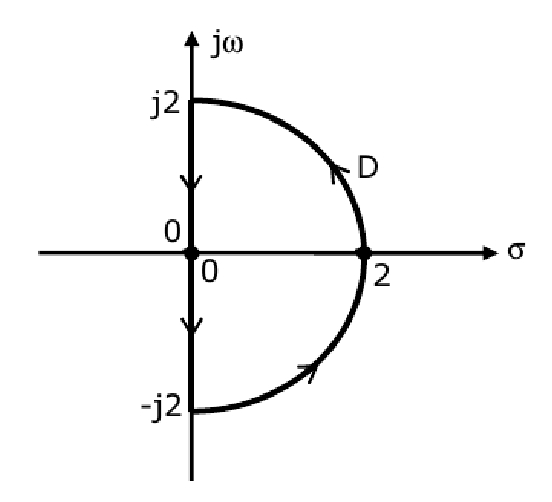
\includegraphics[width=\columnwidth]{./figs/ec2007.eps}
%\caption{}
%\label{fig:ec2018}
%\end{figure}
\item Find
\begin{equation}
\ointctrclockwise\limits_{\abs{z-j}=2}\frac{1}{z^2-1}\,ds
\end{equation}

\item Find $\res{z=0} \frac{\sin z}{z^8}$


\item Let $\Gamma$ denote the boundary of the square whose sides lies along $ x= \pm 1$ and $y= \pm 1$, where $\Gamma$ is described in the positive sense.
Find
\begin{equation}
\ointctrclockwise\limits_{\Gamma}\frac{z^2}{2z + 3} dz
\end{equation}
%Then the value of $ \int\limits_{\Gamma}$ is
%
%\begin{enumerate}[(A)]
%
%\item $
%\frac{\pi i}{4}
%$
%
%\item $
%2 \pi i
%$
%
%\item $
%0$
%
%\item $
%-2 \pi i
%$
%
%\end{enumerate}

\item Evaluate $\int\limits_{0}^{2 \pi} \frac{d \theta}{a+b \cos \theta}$
 %= \frac{2 \pi}{\sqrt{a^2+b^2}}, a>b>0. $

\item For the function $f(z)=\frac{1-e^{-z}}{z}$, the point $z=0$ is


\begin{enumerate}%[(A)]

\item 
an essential singularity

\item 
a pole of order zero

\item 
a pole of order one

\item 
a removable singularity

\end{enumerate}

\item Find
\begin{equation}
\ointctrclockwise\limits_{\abs{z}=4} \frac{dz}{z^2-1}
\end{equation}

%The value of the integral $ \oint\limits_{c} \frac{dz}{z^2-1}$, $ C :\ \mid z \mid =4$ is equal to
%
%\begin{enumerate}[(A)]
%
%\item $
%\pi i
%$
%
%\item $
%0
%$
%
%\item $
%- \pi i
%$
%
%\item $
%2 \pi i
%$
%
%\end{enumerate}

\item Evaluate 
\begin{equation}
\ointctrclockwise\limits_{\abs{z-\j}=\frac{7}{2}} \frac{e^{\frac{1}{z^2}}}{z^2+1}dz
\end{equation}

%the integral $\int\limits_{C}\frac{e^{\frac{1}{z^2}}}{z^2+1} dz ;\ C : \ \mid z-i \mid = \frac{7}{2} $ ,where integration is to be taken counterclockwise.

\item Construct an analytic function $f(z)$ of which the real part is
$u(x,y)=2xy+ \cos hx \sin y $ , given that $f(0)=0$.

\item The function $ \sin z$ is analytic in

\begin{enumerate}

\item $
C \cup \lbrace \infty \rbrace
$

\item 
$C$ except on the negative real axis.

\item $
C-\lbrace 0 \rbrace
$

\item $
C
$

\end{enumerate}
                                                                                                                                                                        
\item If $f(z)=z^3$ , then it

\begin{enumerate}[(A)]

\item 
has an essential singularity at $z=\infty$

\item 
has a pole of order $3$ at $z=\infty$

\item 
has a pole of order $3$ at $z=0$

\item 
is analytic at $z=\infty$

\end{enumerate}

\item The function $f(z) = {\mid z \mid}^2 $ is


\begin{enumerate}

\item 
differentiable everywhere

\item 
differentiable only at the origin

\item 
not differentiable anywhere

\item 
differentiable on real x-axis

\end{enumerate}

\item Evaluate

$\int\limits_{- \infty}^{\infty} \frac{x \sin \pi x}{x^2+2x+5} dx $

using the method of residues.

\item Let $T$ be any circle enclosing the origin and oriented counter-clockwise.
Find $ \int\limits_{\Gamma} \frac{\cos z}{z^2} dz $ 

%\begin{enumerate}
%
%\item $
%2 \pi i
%$
%
%\item $
%0
%$
%
%\item $
%-2 \pi i
%$
%
%\item 
%undefined
%
%\end{enumerate}


\item For the function $f(z) = \sin \frac{1}{z} , z=0 $ is a

\begin{enumerate}

\item 
removable singularity

\item 
simple pole

\item 
branch point

\item 
essential singularity

\end{enumerate}


\item Evaluate the integral 

$\int\limits_{- \infty}^{\infty} \frac{dx}{{(x^2+a^2)}^2} , a>0 $,

by the method of residue calculus.

\item Consider a function $f(z)=u + \j v$ defined on $ \abs{z - \j} < 1 $ where $ u,v $ are real valued functions of $ x,y $. Then $f(z)$ is analytic for $u$ equals to

\begin{enumerate}

\item $
x^2+y^2
$

\item $
\ln (x^2+y^2)
$

\item $
e^{xy}
$

\item $
e^{x^2-y^2}
$

\end{enumerate}

\item At $z=0$ , the function $f(z)=z^2\bar{z}$


\begin{enumerate}

\item 
does not satisfy Cauchy-Reimann equations

\item 
satisfies Cauchy-Reimann equations but is not differentiable 

\item 
is differentiable

\item 
is analytic

\end{enumerate}

\item Let $\gamma$ be the curve : $ r=2+4 \cos \theta , (0 \leq \theta \leq 2\pi)$. If $ I_{1}=\int\limits_{\gamma} \frac{dz}{z-1}$ and $I_{2}= \int\limits_{\gamma}\frac{dz}{z-3}$ then

\begin{enumerate}

\item $
I_{1}=2I_{2}
$

\item $
I_{1}=I_{2}
$

\item $
2I_{1}=I_{2}
$

\item $
I_{1}=0, I_{2} \neq 0
$

\end{enumerate}

\item Let $f(z)$ be an analytic function with a simple pole at $z=1$ and a double pole at $z=2$ with residues $1$ and $-2$ respectively. Further if $f(0)=0$, $f(3)=-\frac{3}{4}$ and $f$ is bounded as $z\rightarrow \infty $ , then $f(z)$ must be

\begin{enumerate}

\item $
z(z-3)-\frac{1}{4}+\frac{1}{z-1}-\frac{2}{z-1}+\frac{1}{(z-2)^2}
$

\item $
-\frac{1}{4}+\frac{1}{z-1}-\frac{2}{z-2}+\frac{1}{(z-2)^2}
$

\item $
\frac{1}{z-1}-\frac{2}{z-2}+\frac{5}{(z-2)^2}
$

\item $
\frac{15}{4}+\frac{1}{z-1}+\frac{2}{z-2}-\frac{7}{(z-2)^2}
$

\end{enumerate}

\item An example of a function with a non-isolated essential singularity at $z=2$ is

\begin{enumerate}

\item $
\tan \frac{1}{z-2}
$

\item $
\sin \frac{1}{z-2}
$

\item $
e^{-(z-2)}
$

\item $
\tan \frac{z-2}{z}
$

\end{enumerate}

\item Find $I= \int\limits_{c}\frac{\cot(\pi z)}{(z-\j)^2}dz$ , where $C$ is the contour $4x^2+y^2=2$ (counter clock-wise).
%Then $I$ is equal to
%
%\begin{enumerate}
%
%\item $
%0
%$
%
%\item $
%-2 \pi i
%$
%
%\item $
%2 \pi i \Big(\frac{\pi}{\sin h^2 \pi} - \frac{1}{\pi}\Big)
%$
%
%\item $
%- \frac{2 {\pi}^2 i}{\sin h^2 \pi}
%$
%
%\end{enumerate}

\item $\int_{0}^{2 \pi}\frac{d \theta}{13-5 \sin \theta}= $


%\begin{enumerate}
%
%\item $
%-\frac{\pi}{6}
%$
%
%\item $
%-\frac{\pi}{12}
%$
%
%\item $
%\frac{\pi}{12}
%$
%
%\item $
%\frac{\pi}{6}
%$
%
%\end{enumerate}


\item For the positively oriented unit circle, find $\oint\limits_{\mid z \mid = 1 } \frac{2 \text{Re}(z)}{z+2} dz $
 
%\begin{enumerate}
%
%\item $
%0
%$
%
%\item $
%\pi i
%$
%
%\item $
%2 \pi i
%$
%
%\item $
%4 \pi i
%$
%
%\end{enumerate}

\item The number of zeroes, counting multiplicities, of the polynomial $z^5+3z^3+z^2+1$ inside the circle $ \mid z \mid =2 $ is


\begin{enumerate}

\item $
0
$

\item $
2
$

\item $
3
$

\item $
5
$

\end{enumerate}


\item Consider the functions $f(z)=x^2+\j y^2$ and $g(z)=x^2+y^2+ \j x y$. At $z=0$,

\begin{enumerate}

\item
$f$ is analytic but not $g$

\item
$g$ is analytic but not $f$

\item
both $f$ and $g$ are analytic

\item
neither $f$ nor $g$ is analytic


\end{enumerate}


\item Let $\gamma$ be a simple closed curve in the complex.Then the set of all possible values of
$\oint\limits_{\gamma} \frac{dz}{z(1-z^2)}$ is

\begin{enumerate}

\item $
\lbrace 0, \pm \pi \j \rbrace
$

\item $
\lbrace 0, \pi \j, 2 \pi \j \rbrace
$

\item $
\lbrace 0, \pm \pi \j, \pm 2 \pi \j \rbrace
$

\item $
\lbrace 0 \rbrace
$


\end{enumerate}


\item The principal value of the improper integral $\int\limits_{-\infty}^{\infty} \frac{\cos x}{1+x^2} dx $ is

\begin{enumerate}

\item $
\frac{\pi}{e}
$

\item $
\pi e
$

\item $
\pi + e
$

\item $
\pi - e
$

\end{enumerate}

\item The number of roots of the equation $z^5-12z^2+14=0$ that lie in the region 
$ \lbrace z \in C : 2 \leq \mid z \mid < \frac{5}{2} \rbrace $ is

\begin{enumerate}

\item $
2
$

\item $
3
$

\item $
4
$

\item $
5
$

\end{enumerate} 




\item Find the value of $\int\limits_{0}^{2 \pi} \exp ( e^{\j \theta} - \j \theta) \,d \theta $ 


%\begin{enumerate}
%
%\item $
%2 \pi i
%$
%
%\item $
%2 \pi 
%$
%
%\item $
%\pi 
%$
%
%\item $
%i \pi
%$
%
%\end{enumerate}

\item The sum of the residues at all the poles of $ f(z) = \frac{\cot \pi z}{(z+a) ^ 2}$ , where $a$ is a constant, $(a \neq 0, \pm 1, \pm 2,......)$ is

\begin{enumerate}

\item $
\frac{1}{\pi} \sum\limits_{n= -\infty}^{\infty} \frac{1}{(n+a)^2} - \pi \text{cosec}^2 \pi a
$


\item $
-\frac{1}{\pi} \sum\limits_{n= -\infty}^{\infty} \frac{1}{(n+a)^2} + \pi \text{cosec}^2 \pi a
$


\item $
-\frac{1}{\pi} \sum\limits_{n= -\infty}^{\infty} \frac{1}{(n+a)^2} - \pi \text{cosec}^2 \pi a
$


\item $
\frac{1}{\pi} \sum\limits_{n= -\infty}^{\infty} \frac{1}{(n+a)^2} + \pi \text{cosec}^2 \pi a
$

\end{enumerate}

\item Which of the following is not the real part of an analytic function?

\begin{enumerate}

\item $
x^2-y^2
$

\item $
\frac{1}{1+x^2+y^2}
$

\item $
\cos x \cos h y
$

\item $
x+ \frac{x}{x^2+y^2}
$

\end{enumerate}

\item Let $f(z)$ be an analytic function. Then the value of $\int_{0}^{2 \pi} f(e^{\j t}) \cos (t) dt $ equals

\begin{enumerate}

\item $
0
$

\item $
2 \pi f(0) 
$

\item $
2 \pi f^\prime(0) 
$

\item $
\pi f^\prime(0)
$

\end{enumerate}

\item Let $f(z)=2z^2-1$. Then the maximum value of $ \mid f(z) \mid $ on the unit disc 
$ D= \lbrace z \in C :  \abs{z} \leq 1 \rbrace $ equals 


\begin{enumerate}

\item $
1
$

\item $
2
$

\item $
3
$

\item $
4
$

\end{enumerate} 


\item Let $S$ be the positively oriented circle given by $  \abs{z- 3 \j} =2 $. Find the value of 
$\int\limits_{S} \frac{dz}{z^2+4} $ 


%\begin{enumerate}
%
%\item $
%-\frac{\pi}{2}
%$
%
%\item $
%\frac{\pi}{2}
%$
%
%\item $
%-\frac{i \pi}{2}
%$
%
%\item $
%\frac{i \pi}{2}
%$
%
%\end{enumerate}
%
%\begin{center}
%
%\centering\textbf{Statement for Linked Answer Questions $34$ and $35 $:}
%
%\end{center}




\item Let $f(z) = \cos z - \frac{\sin z}{z} $ for non-zero $z \in \mathbb{C}$ and $f(0)=0$. Also,let $g(z)=\sin hz $ for $z \in \mathbb{C}$. Then $f(z)$ has a zero at $z=0$ of order

\begin{enumerate}

\item $
0
$

\item $
1
$

\item $
2
$

\item 
greater than $2$


\end{enumerate}

\item Refer to the previous question for $f(z)$ and $g(z)$.  Then $\frac{g(z)}{z f(z)}$ has a pole at $z=0$ of order

\begin{enumerate}

\item $
1
$

\item $
2
$

\item $
3
$

\item 
greater than $3$


\end{enumerate}


\item For the function $ f(z)= \sin \brak{ \frac{1}{\cos\brak{\frac{1}{z}}} }$ , the point $z=0$ is

\begin{enumerate}

\item 
a removable singularity

\item 
a pole

\item 
an essential singularity

\item 
a non-isolated singularity

\end{enumerate}

%\begin{center}
%
%%\centering\textbf{Statement for Linked Answer Questions $37$ and $38$:}
%
%\end{center}



\item Consider the function $f(z) = \frac{e^{\j z}}{z(z^2+1)}$. The residue of $f$ at the isolated singular point in the upper half plane 
$ \lbrace z=x+\j y : y>0 \rbrace $ is

\begin{enumerate}

\item $
-\frac{1}{2e}
$

\item $
-\frac{1}{e}
$

\item $
\frac{e}{2}
$

\item $
2
$

\end{enumerate}

\item The Cauchy Principal Value of the integral $\int\limits_{-\infty}^{\infty} \frac{\sin x dx}{x(x^2+1)} $ is


\begin{enumerate}

\item $
-2 \pi(1+2 e^{-1})
$

\item $
\pi(1+e^{-1})
$

\item $
2 \pi(1+e) 
$

\item $
- \pi(1+e^{-1})
$

\end{enumerate}

\item Let $ I=\int\limits_{C} \frac{f(z)}{(z-1)(z-2)} dz$, where $f(z)= \sin \frac{\pi z}{2} + \cos \frac{\pi z}{2} $ and $C$ is the curve $  \abs{z}  =3 $ oriented anti-clockwise. Find the value of $I$ 

%\begin{enumerate}
%
%\item $
%4 \pi i
%$
%
%\item $
%0
%$
%
%\item $
%- 2 \pi i
%$
%
%\item $
%- 4 \pi i
%$
%
%\end{enumerate}

\item Let $ f : \mathbb{C} \rightarrow \mathbb{C} $ be analytic except for a simple pole at $z=0$ an let $ g : \mathbb{C} \rightarrow \mathbb{C} $ be analytic.
Then, the value of $\dfrac{\res{z=0} \lbrace f(z)g(z)\rbrace }{\res{z=0} f(z)} $ is

\begin{enumerate}

\item $
g(0)
$

\item $
g'(0)
$

\item $
\lim\limits_{z \to 0} z f(z)
$
       
\item $
\lim\limits_{z \to 0} z f(z) g(z)
$

\end{enumerate}

\item Let $C$ be the contour $ \abs{z}= 2$ oriented in the anti-clockwise direction. The value of the integral $\oint\limits_{C} z e ^{\frac{3}{z}} dz $ is

\begin{enumerate}

\item $
3 \pi \j
$

\item $
5 \pi \j
$

\item $
7 \pi \j
$

\item $
9 \pi \j
$

\end{enumerate}

\item The function $f(z)= { \abs{z}}^2 + \j \bar{z} + 1 $ is differentiable at

\begin{enumerate}

\item $
\j
$

\item $
1
$

\item $
-\j
$

\item 
no point in $ \mathbb{C}
$

\end{enumerate}

\item The inverse Laplace transform of $ \frac{2s^2-4}{(s-3)(s^2-s-2)} $ is

\begin{enumerate}

\item $
(1+t)e^{-t} + \frac{7}{2} e^{-3t} 
$

\item $
\frac{e^t}{3} + t e^{-t} + 2t
$

\item $
\frac{7}{2} e^{3t} - \frac{e^{-t}}{6} - \frac{4}{3} e^{2t}
$

\item $
\frac{7}{2} e^{-3t} - \frac{e^{t}}{6} - \frac{4}{3} e^{-2t}
$

\end{enumerate}

\item The maximum modulus of $ e^ {z^2} $ on the set $S = \lbrace z \in \mathbb{C} : 0 \leq \text{Re}(z) \leq 1, 0 \leq \text{Im}(z) \leq 1 \rbrace $ is

\begin{enumerate}

\item $
\frac{2}{e}
$

\item $
e
$

\item $
e+1
$

\item $
e^2
$

\end{enumerate}


\item Let $\Omega = \lbrace z \in \mathbb{C} : \text{Im}(z) > 0 \rbrace $ and let $C$ be a smooth curve lying in $\Omega $ with initial point $ -1 + 2\j$ and final point $1+2\j$. The value of $ \int\limits_{C} \frac{1+2z}{1+z} dz $ is

\begin{enumerate}

\item $
4-\frac{1}{2} \ln 2+ \j \frac{\pi}{4}
$

\item $
-4+\frac{1}{2} \ln 2+ \j \frac{\pi}{4}
$

\item $
4+\frac{1}{2} \ln 2- \j \frac{\pi}{4}
$

\item $
4-\frac{1}{2} \ln 2+ \j \frac{\pi}{2}
$

\end{enumerate}

\item If $a \in \mathbb{C} $ with $ \mid a \mid < 1 $, then the value of
$$\frac{(1- { \abs{a}  }^2)}{\pi} \int\limits_{\Gamma} \frac{ \abs{dz}}{{\abs{z+a}  }^2}, $$
where $\Gamma$ is the simple closed curve $ \mid z \mid =1 $  taken with the positive orientation, is 
$\rule{3cm}{0.15mm}$


\item Let $C = \lbrace z \in \mathbb{C} :  \abs{z-\j} =2 \rbrace $. Then $ \frac{1}{2 \pi} \oint_{C} \frac{z^2-4}{z^2+4} dz $ is equal to $ \rule{3cm}{0.15mm}$

\item The value of $\frac{\j}{4 - \pi} \int_{\mid z \mid =4} \frac{dz}{z \cos(z)}$ is equal to $\rule{3cm}{0.15mm}$

\item Let $ \gamma =\lbrace z \in \mathbb{C} :  \abs{z}=2 \rbrace $ be oriented in the counter-clockwise direction. Let
$$ I = \frac{1}{2 \pi \j} \oint\limits_{\gamma} z^7 \cos \Big(\frac{1}{z^2}\Big) dz. $$
Then,the value of $I$ is equal to $\rule{3cm}{0.15mm}$ 

\item Let $f(z)=(x^2+y^2)+\j 2 xy $ and $g(z)= 2 xy + \j (y^2-x^2) $ for $z= x+ \j y \in \mathbb{C} $. Then, in the complex plane $\mathbb{C}$.

\begin{enumerate}

\item
$f$ is analytic and $g$ is NOT analytic.

\item
$f$ is NOT analytic and $g$ is analytic.

\item
neither $f$ nor $g$ is analytic.

\item
both $f$ and $g$ are analytic.

\end{enumerate}

\item Let $C$ be the simple,positively oriented circle of radius $2$ centered at the origin in the complex plane. Then find

$$\frac{2}{\pi \j} \int\limits_{C} \Bigg( z e^{\big(\frac{1}{z}\big)} + \tan \bigg(\frac{z}{2} \bigg) + \frac{1}{(z-1)(z-3)^2} \Bigg) dz $$ . 

\item Let $\Gamma $ be the circle given by $z=4 e^{\j \theta}$, where $\theta$ varies from $ 0 $ to $ 2 \pi $. Find

$$ \oint_{\Gamma} \frac{e^z}{z^2-2z} dz = $$

%\begin{enumerate}
%
%\item $
%2 \pi i (e^2-1)
%$
%
%\item $
%\pi i (1-e^2)
%$
%
%\item $
%\pi i (e^2-1)
%$
%
%\item $
%2 \pi i (1-e^2)
%$
%\end{enumerate}

\item Let $f(z)= z^3e^{z^2}$ for $z \in \mathbb{C}$ and let $\Gamma$ be the circle $z= e^{\j \theta}$, where $\theta$ varies from $0$ to $4 \pi $. Then

$$ \frac{1}{2 \pi \j} \oint_{\Gamma} \frac{f'(z)}{f(z)} dz= \rule{3cm}{0.15mm}.$$


\end{enumerate}


\end{document}


